\documentclass[12pt,a4paper]{article}
\usepackage[utf8]{inputenc}
\usepackage[T1]{fontenc}
\usepackage{amsmath}
\usepackage{textcomp}

\usepackage{geometry}
\geometry{a4paper,left=25mm,right=25mm, top=2cm, bottom=2cm} 

\usepackage{graphicx} %fuer bilder

\usepackage{verbatim}


\usepackage{pgfplots}

 \usepackage{mathptmx}
 \usepackage[scaled=.90]{helvet}
 \usepackage{courier}



\usepackage{listings}
\usepackage{color}

\usepackage{float}
 
\definecolor{dkgreen}{rgb}{0,0.6,0}
\definecolor{gray}{rgb}{0.5,0.5,0.5}
\definecolor{mauve}{rgb}{0.58,0,0.82}

\pagestyle{empty}
\lstset{numbers=left,language=C++}
\lstset{showstringspaces=false,
basicstyle=\ttfamily\footnotesize,
breaklines=true,
tabsize=3,
commentstyle=\color{dkgreen},      % comment style
inputencoding={ansinew},
title=\lstname %zeigt titel der datei an
}

\usepackage{pdfpages} % fuer pdfs
\usepackage{hyperref} % fuer url

%keine einrückungen bei absatz
\parindent 0pt

\begin{document}
\title{Übung 11}
\author{Reinhard Penn, Bernhard Selymes}
\date{Juni 2015}

\normalsize

%Beginn des Dokuments

\newcommand{\srcpath}{../../src}
\newcommand{\simpath}{../../sim}

%Angabe
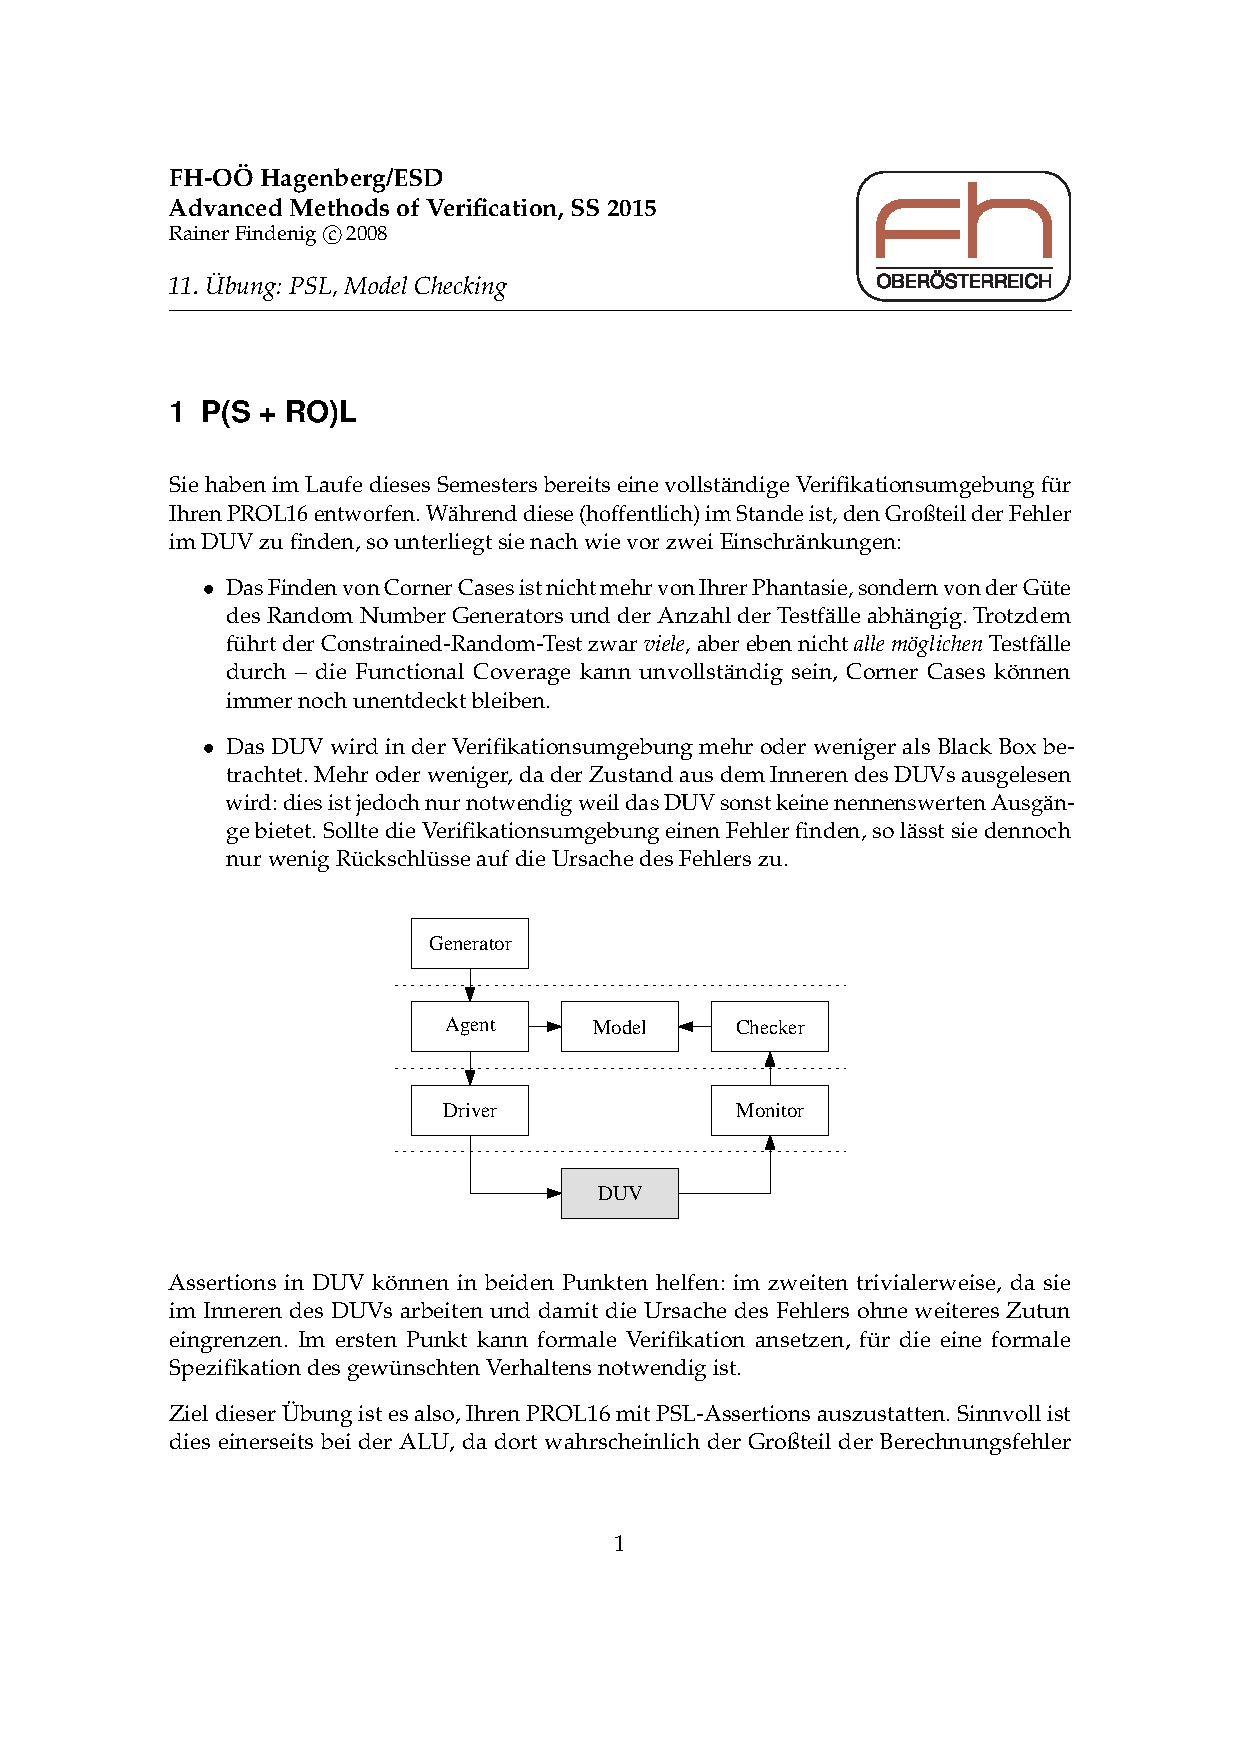
\includepdf[pages=-]{../Angabe.pdf}

\section{P(S + RO)L}
\subsection{ALU}
Bei der ALU wurden die einzelnen ALU-Befehle durchgegangen und je nach Befehl überprüft ob das Ergebnis stimmt. Die Flags wurden extra überprüft und für die ALU-Befehle die zusammen gehören in einer Property überprüft.

\subsection{Control}
Zyklus 1 und 2 werden und die einzelnen Befehle werden extra überprüft. Es wird überprüft ob die Output-Flags richtig gesetzt werden. Die Default-Zuweisung für die Flags werden nicht überprüft, da dies sehr aufwendig ist.

\section{Theorie}

\begin{itemize}
	\item Bei Vacuity handelt es sich um nichts aussagende/leere Assertions. Ein Beispiel dafür wäre "always (a -> next b)", unter der Annahme das a nie zutrifft. Da a immer falsch ist, ist es irrelevant was auf der rechten Seite steht, man kann den bestehenden Ausdruck durch einen beliebigen boolschen Ausdruck ersetzen.
Dieses Konzept ist wichtig, da damit mögliche Fehler aufgedeckt werden können. Nimmt man das obige Beispiel, erwartete sich die Person, die die Assertion schrieb, dass a irgendwann wahr ist.
Es ist auch für andere Logiken wichtig, die obige Bedingung kann man ebenso in LTL/CTL beschreiben.
  \item Signalverläufe
		\begin{itemize}
			\item x: 0 -> 0 -> 0 -> 0 -> 0 -> 0 …
			\item x: 0 -> 0 -> 0 -> 0 -> 0 -> 0 …
			\item x: 0 -> 1 -> 1 -> 0 -> 0 -> 0 … \\
						y: 0 -> 1 -> 0 -> 0 -> 1 -> 0 …
			\item x: 0 -> 1 -> 1 -> 0 -> 1 -> 0 … \\
						y: 0 -> 1 -> 0 -> 0 -> 1 -> 0 …
		\end{itemize}
	\item Die schwache Version ergibt wenig Sinn, da sie immer wahr sein würde. Denn nach der Simulation könnte die \texttt{eventually} Bedingung noch erfüllt werden und im Zweifel ist die schwache Version wahr.
	\item Es wird in einem Initialzustand begonnen. Dieser Zustand kommt zu den neuen Zuständen hinzu.
Danach wird überprüft ob ein neuer Zustand eine Assertion verletzt. Falls eine Assertion verletzt wurde, wird ein Gegenbeispiel ausgegeben. Falls keine verletzt wurde, werden alle nachfolgenden Zustände ermittelt. Dies geschieht indem bei den zuvor überprüften Zuständen alle möglichen Eingabekombinationen angelegt werden. Sind bei den Nachfolgezuständen neue Zustände dabei werden diese wieder überprüft und ihre Nachfolger erzeugt. Sobald keine neuen Zustände gefunden werden, wird der Beweis ausgegeben.
\end{itemize}

\section{Model Checking: Anwendung}

\subsection{Mutex}
Anhand des kombinierten Graphen kann man erkennen, dass alle Bedingungen erfüllt werden. Es gibt keinen Zustand C1C2 und nach einem T Zustand kommt immer ein C Zustand.

\begin{figure}[!htb]%
\centering
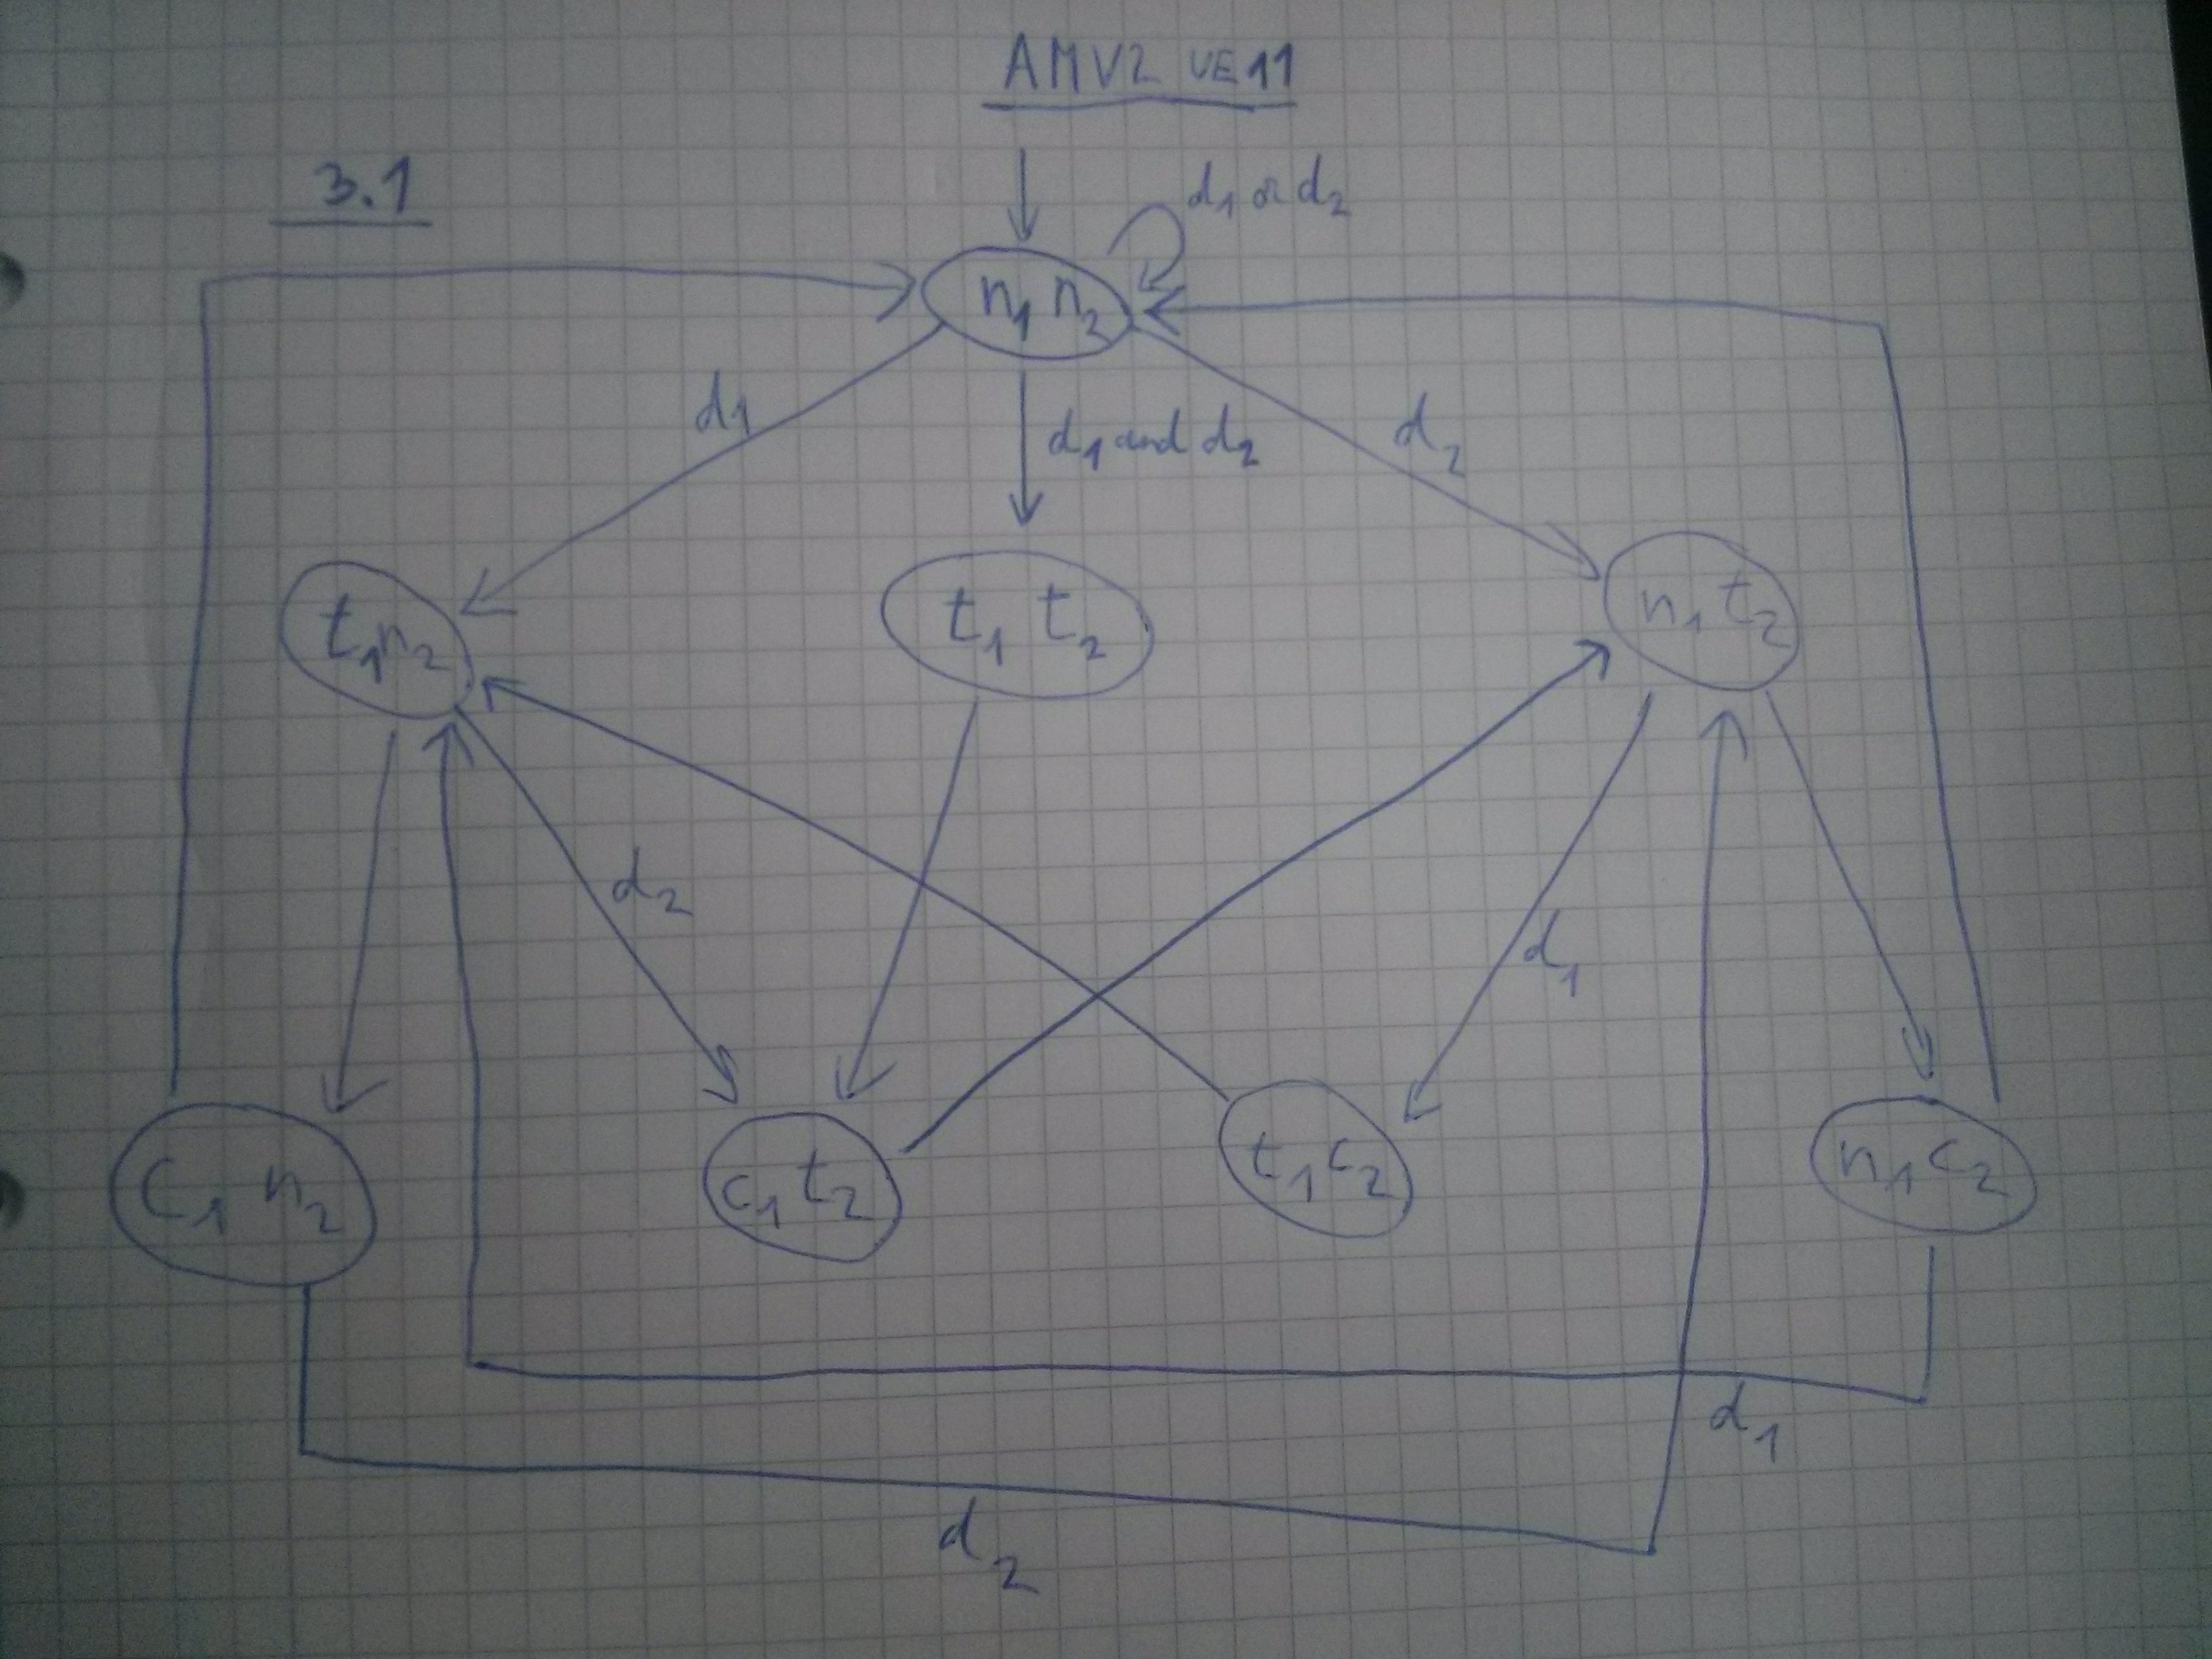
\includegraphics[width=\textwidth]{3_1}%
\caption{Mutex Graph}%
\label{}%
\end{figure}

\subsection{Mutex, Implementierung 2}
Man kann anhand des Zustandsgraphen erkennen das die erste Bedingung nicht mehr erfüllt wird, denn es gibt nun einen Zustand C1C2 indem beide kritischen Zustand sind. Die letzten beiden Bedingungen werden jedoch weiterhin erfüllt. \\
Gegenbeispiel: N1N2->(d1=1,d2=1)->T1T2->C1C2->N1N2

\begin{figure}[!htb]%
\centering
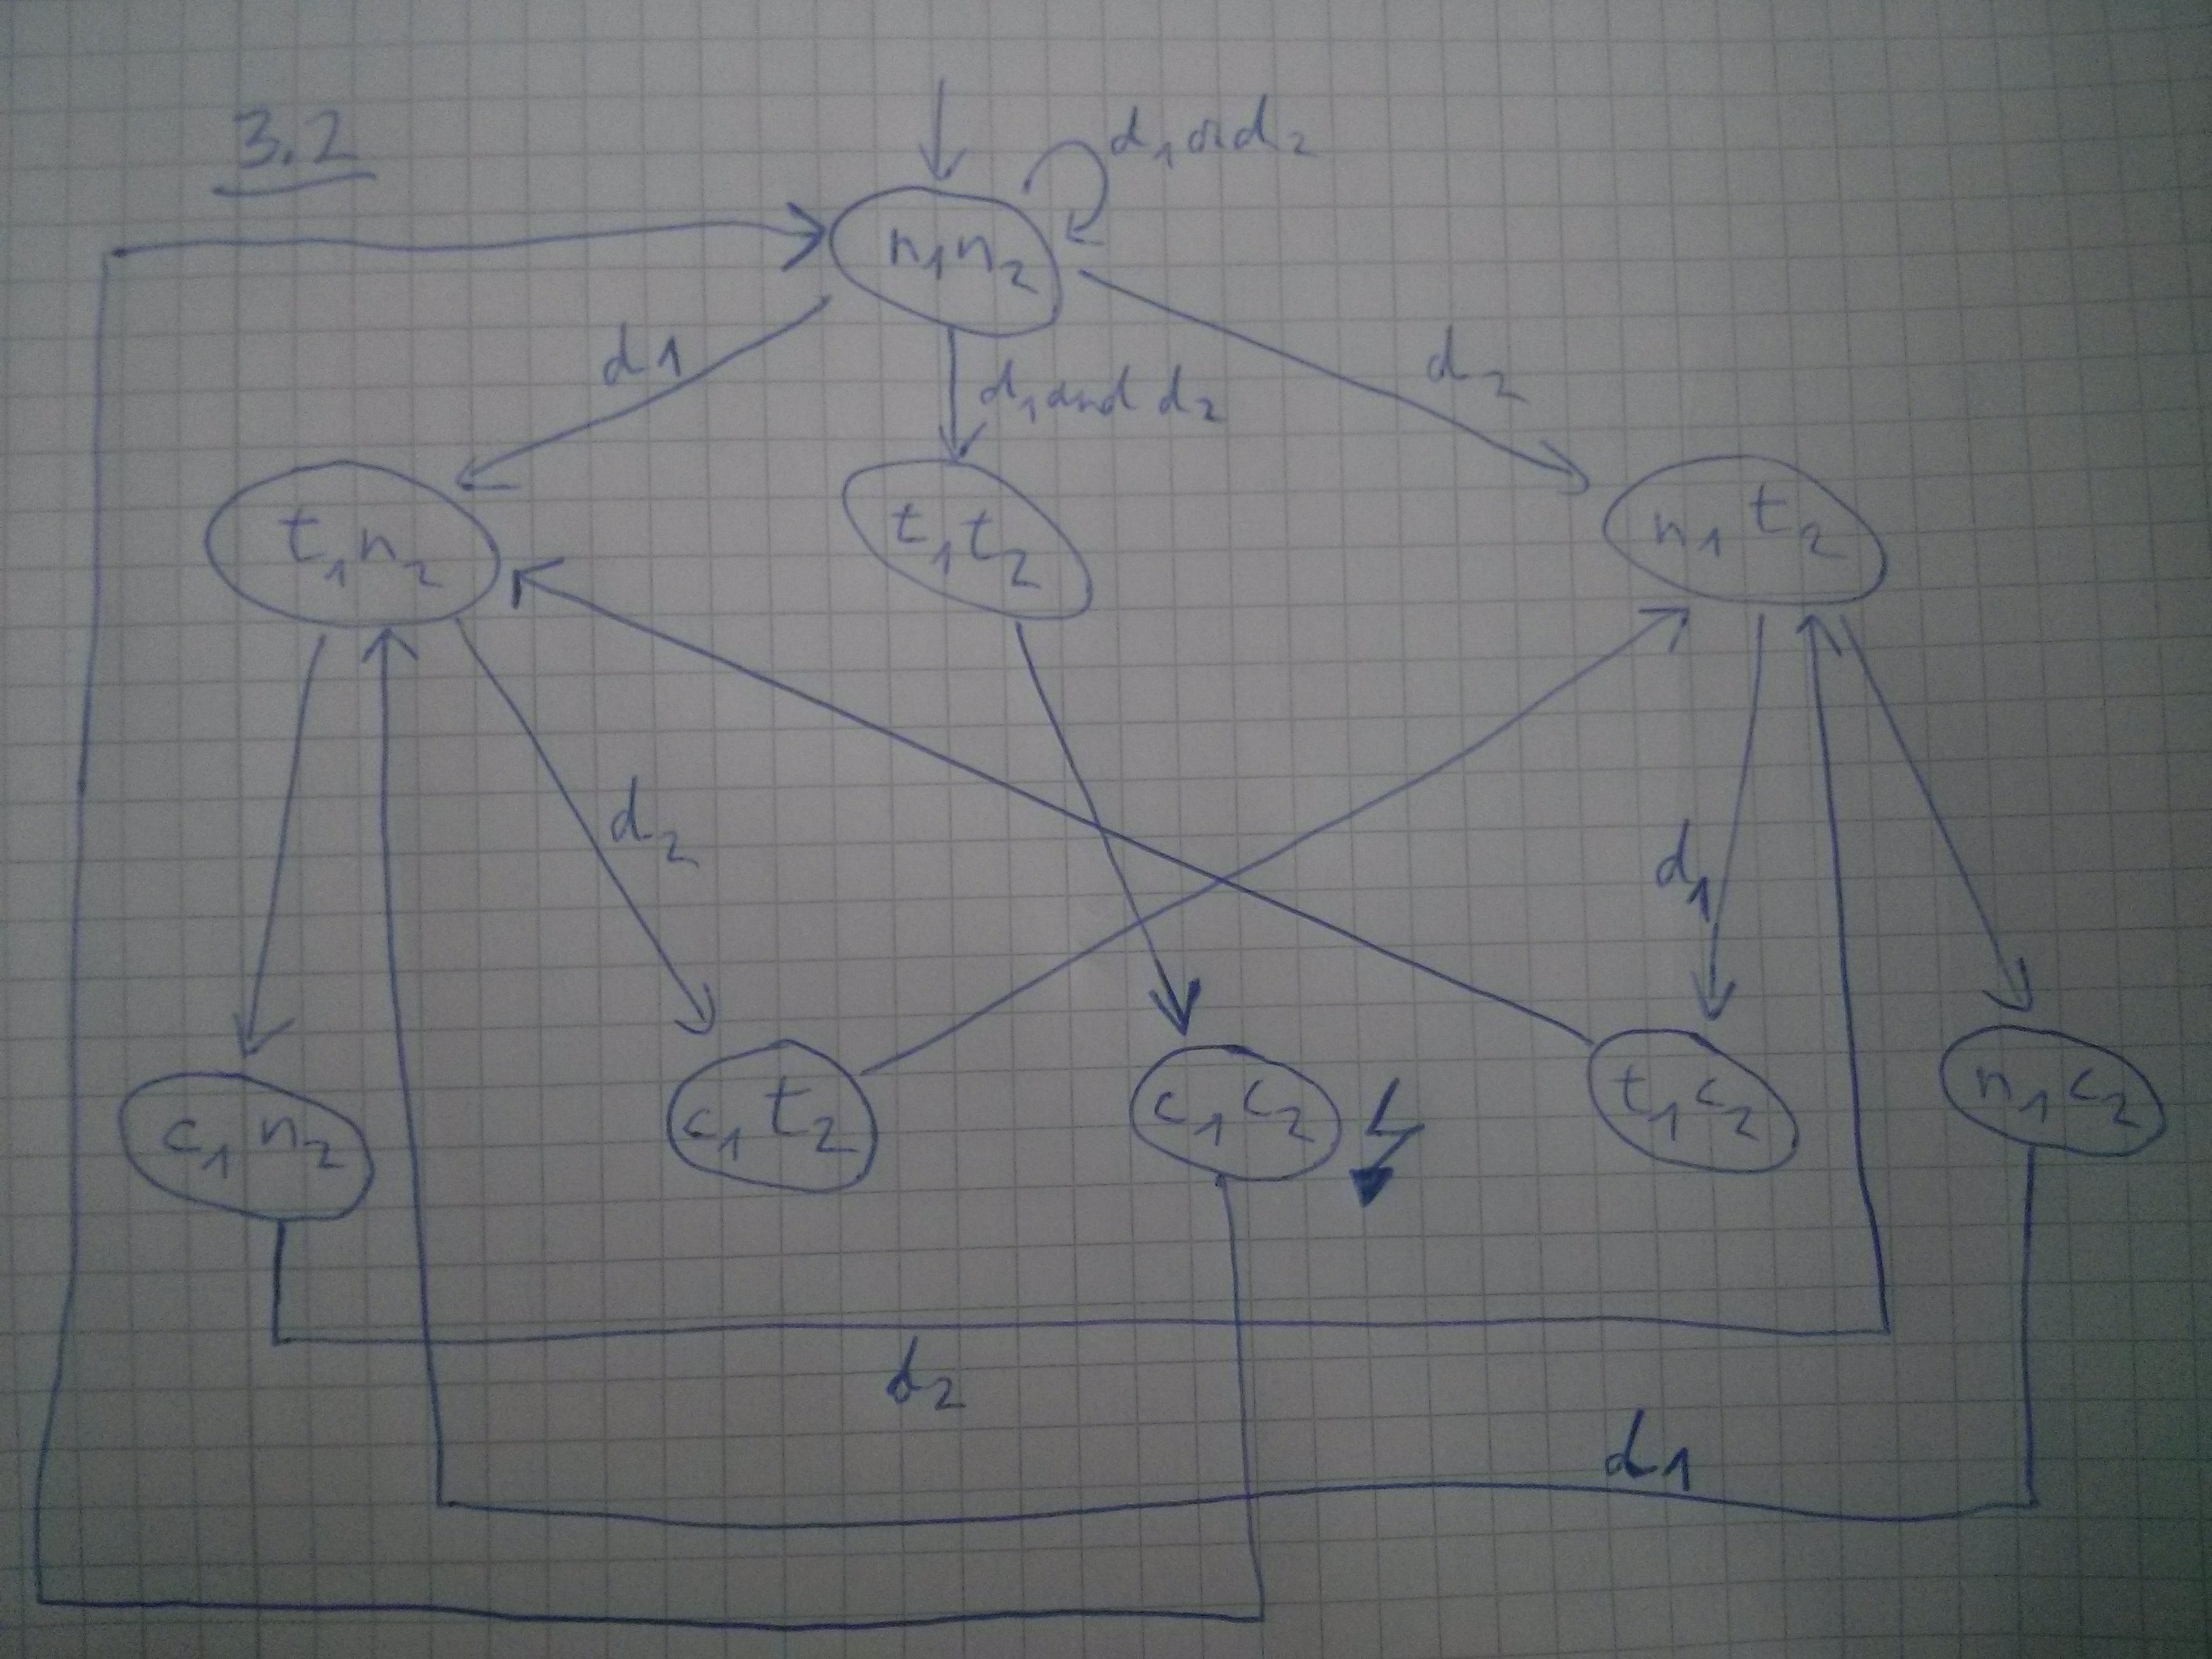
\includegraphics[width=\textwidth]{3_2}%
\caption{Mutex, Implementierung 2 Graph}%
\label{}%
\end{figure}

\end{document}
